%!TEX root = ./rules-working.tex
%LTeX: enabled=false

\rulechapter{Bombing Attacks}

\label{rules:bombing-attacks}

This chapter details the methods used to resolve air to ground attacks with ballistic bombs. Aiming and being at the proper release point as described in Rule \ref{rule:release-points} is required in order to declare a bombing attack.

\paragraph{Bombing Parameters.} Aircraft may drop bombs from level or diving flight while on a LOA to the target. Aiming and reaching the proper release point for the attack must occur from the same flight type. A level bomb attack requires level flight aiming, and a diving attack requires aiming while in diving flight. The release point charts differ for level and diving bomb attacks.

\paragraph{BB Weapon Final Attack Strengths.} The final attack of a bombing attack is determined as follows:

\begin{itemize}

    \item 
For HE, Fire and Napalm bombs: Sum the attack strengths of all the individual bombs released at the time of the attack. Take two thirds of that number (rounded up) and that is the FAS. (As bombs are dropped in strings, some will fall short of or past the target, so the full values are not used.)

    \item For Cluster bombs: Sum the attack strengths directly and that is the FAS. (The vast number of bomblets the cluster bombs release makes up for the ones falling long or short).

\end{itemize}

\paragraph{Bomb Types.} BB class weapons are either LOW DRAG or HIGH DRAG weapons depending on type and/or whether they are or are not fitted with parachute or pop-open fin (snake-eye type) retardation devices.

Low drag weapons are those of normal aerodynamic shape with stabilizing fins; mainly HE, AP, AT, cluster bombs and FAE bombs. High drag weapons are those which lack fins and tumble when dropped (napalm and fire bombs), or runway cratering weapons, or any of the above Low drag weapons that have been fitted with retardation devices.

High drag weapons use different release parameters than low drag ones as indicated on the release point tables. High drag weapons were developed to allow T-level laydown attacks as described below.

\paragraph{Multiple Bombs.} When a bombing attack is declared, any number of weapons of the same type may be dropped; meaning all are either low or high drag AND all are of one class (HE or AP for example). Different sized weapons of the same type may be dropped together.

\paragraph{Bomb Time Of Fall.} When a bomb attack is declared, it does not occur instantly; it takes time for the bombs to reach the target. To reflect this; place a marker on the line of approach under the aircraft the instant it declares the attack. For every FP the aircraft expends after the marker is placed, advance the marker one hex down the line. Do this until the marker reaches the target hex or the aircraft ceases moving (ignore bomb altitude).

If the bombs reach the target while the aircraft is moving, the attack is resolved at that instant. If the aircraft is destroyed for any reason prior to the bombs hitting, they are unaffected and can continue moving down the line for as many points as the aircraft had left. If they do not reach the target, the attack is resolved at the end of the turn after all aircraft have moved.  Targets may continue to function normally until the instant of attack (for example, AAA guns can track and fire until hit).

\paragraph{Carriage Speed Restrictions.} The maximum safe speed which bombs may be dropped at is High Transonic. The maximum safe speed for carrying bombs on external weapons racks or stations is 6.0.

If the safe carriage speed is ever exceeded, some of the weapon fuze mechanisms will suffer damage. To reflect this, when an attack is made dropping bombs whose safe carriage speed was exceeded use the following:

\begin{itemize}
    \item If a single weapon was dropped, it duds (automatically misses) if the attack roll is odd.
    \item If multiple weapons were dropped, halve the FAS determined for the group of bombs.
\end{itemize}

Additionally, if the aircraft is above high transonic speed when the bomb attack is made, some of the bombs may pitch up and bounce off the aircraft upon release. To reflect this, roll for damage to the aircraft as if it had been hit by a weapon with an attack rating of 1 after declaring the bomb attack.

\paragraph{Additional Bombing Modifiers.} In addition to the usual bombsight, release point, tracking time and aircraft damage level modifiers, the following apply to bombing attacks:

\begin{itemize}
    \item Sticks of Bombs: For every three BB weapons dropped in a single attack subtract one from the attack roll (better target coverage).

    \item Napalm and Fire Bombs: These are not very accurate weapons. For each altitude level greater than one above the target, add one to the attack roll.

    \item Miscellaneous Weapons Effects: Some weapons are more effective against different target types. See the modifiers table under the release point tables for additional modifiers which may apply against targets.
\end{itemize}

\paragraph{Laydown Bombing Attack Runs.} Only aircraft in T-level flight are allowed to execute laydown attack runs. Laydown attacks may only be done with high drag weapons, napalm and fire bombs, runway cratering weapons and area weapon dispenser pods.

The release point of a laydown attack is always the target hex itself and aiming is still required.  Aircraft with computed or advanced sights may attack multiple targets during their run. One target in each of up to three different hexes may be struck.  If the targets are in adjacent hexes, one after another in a row, relative to the aircraft's flight path, aiming is only required on the first target to start the attack and those in the other hexes are attacked using the same modifiers.

If the targets are not in adjacent hexes, aiming is required to be done anew prior to attacking subsequent hexes. The laydown attack run, be it against one or more hexes, is considered to be the single air to ground attack allowed an aircraft per turn.

Exception: Aircraft using an area weapon dispenser pod (WP) are allowed to attack as many hexes as its listed capacity (see weapons tables) in a single run.

\begin{advancedrules}
    
\section{Advanced Bombing Techniques}

The following sections detail bombing techniques that have been developed since World War Two due to the advent of ballistics computing weapons systems.

\subsection{Toss Boming}

Aircraft with computed or advanced sights may “TOSS” low drag bombs at targets by lofting them out of a zoom climb.

\paragraph{Procedure.} Announce the toss attack prior to moving the aircraft. Aiming is required to be done normally by expending HFPs on the line of approach. After aiming is complete, the aircraft may expend VFPs in the zoom climb. The weapons may be released after the expenditure of any VFP.

\paragraph{Toss Release Point.} The release point, in terms of hexes away from the target, is always the sum of the levels zoomed prior to release plus the aircraft's height in levels above the target at the start of the turn.

\paragraph{Toss Restrictions and Modifiers.} Toss bombing may not be done if the release point is more than six hexes away from the target. Toss bombing keeps you further away from point defenses but is less accurate. There is a Toss bomb attack modifier to the die roll of \plus{1} per hex away from the target at release.  

\subsection{Lateral Toss Boming}

This is a variation of toss bombing but done in the horizontal. Aircraft with computed or advanced sights, in T-level flight or level flight not more than one altitude level above the target may do lateral toss bombing. The aircraft uses the turn to “sling” the bombs horizontally at the target, hence the term ”lateral toss”.                              

\paragraph{Procedure.} The aircraft approaches a target not on a line of approach but parallel to one so that it will intersect an actual line of approach. It MUST commence an HT or BT turn so that when it faces, it is on the intersecting LOA pointed at the target. It then continues down the line of approach toward the target and still in the turn. The instant it faces again, the bombs are considered released at the target (even though the aircraft is not facing it anymore).

\paragraph{Aiming.} Aiming is considered to occur while the aircraft is in the turn and facing the target. This is a deliberate exception to the rule that aircraft must be wings level while aiming.

\paragraph{Lateral Toss Release Point.} The release point for lateral toss bombing is one, two or three hexes from the target. Tracking time is not allowed. The modifier for this attack is \plus{2} per hex of range. It is daring but not accurate! \changedin{1C}{1C-figures}{Below is a diagram of}{Figure \ref{figure:lateral-toss-bombing-example} shows an example of a} lateral toss attack. Lateral toss bombing can only be done visually and was developed to allow aircraft to stay low and throw low drag bombs at a target without blowing themselves up.

%!TEX root = ../rules-working.tex
%LTeX: enabled=false

\begin{onecolumnfigure}[h!]

{\bfseries Example of Lateral Toss Attack}

\includegraphics[width=\linewidth]{figures/figure-lateral-toss-bombing-example.pdf}
\end{onecolumnfigure}


\subsection{Offset Aimpoint Bombing}

Aircraft with computed or advanced sights may attack a target whose geographic coordinates (fixes) are known before the mission, without having to see it. This is done by aiming off another prominent location whose coordinates are also known.

\paragraph{Known Target Coordinates.} You may assume that mission planners know the fixes of all bridges, dams, runways, airport facilities, piers, small islands, and any other hex marked on the game map by a black triangle. Scenarios will state if any other target units or counters have had their locations fixed by reconnaissance prior to play.

\paragraph{Offset Aiming Procedure.} To bomb a target with offset aiming, an aircraft must first pass over a known fix, or obtain a radar lock-on to a known fix in order to update its inertial navigation system (present on any aircraft with computed or advanced sights). The update fix must be within 12 hexes of the intended release point. Updates may be obtained while the aircraft is in a turn as long as it is of HT or less rate. The update is automatic upon flying over the fix.

After updating, the aircraft may then position itself on a line of approach to the target and perform level bombing or toss bombing. Aiming is performed on the line of approach to the target but the target does not have to be visually sighted or locked on by radar.

Offset aiming is generally used when adverse weather prevents accurate visual bombing and the target itself is not radar significant but something near it is.

\paragraph{FAS and Modifier Effects.} All normal modifiers for level or toss attacks apply except that the FAS is determined as if the target were a secondary target.

\subsection{Blast and Fragmentation Danger Zones}

%!TEX root = ../rules-working.tex
%LTeX: enabled=false

\addedin{1B}{1B-figures}{

\begin{onecolumnfigure}

\begin{fitheight}{3.2\standardhexwidth}
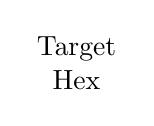
\begin{tikzpicture}
    \setfiguresize{-2.5}{-1.6}{+2.5}{+1.6}
    \drawhex{0}{0}  
    \drawhex{0}{+1}  
    \drawhex{0}{-1}  
    \drawhex{+1}{+0.5}  
    \drawhex{+1}{-0.5}  
    \drawhex{-1}{+0.5}  
    \drawhex{-1}{-0.5}  
    \drawhex[ultra thick,black]{0}{0}
    \node at (0,0) [align=center] {Target\\Hex};
\end{tikzpicture}
\end{fitheight}

\figurecaption{figure:blast-zone}{Blast and Fragmentation Danger Zone.}

\end{onecolumnfigure}
}


HE bombs and other highly destructive weapons have been known to blast their fragments and debris thousands of feet into the air. In fact, attack aircraft bombing from low level have blasted themselves out of the sky so often that tactics and maneuvers are devised with the primary purpose of avoiding the blast zones of weapons dropped.

\paragraph{Blast Zone (BZ) Markers.} BZ markers are used to identify fragmentation danger areas for aircraft. Place a BZ marker in any hex which is:

\begin{itemize}
    \item attacked by HE bombs, Runway Cratering weapons, Rocket Pods or rockets with an unmodified soft FAS of 6 or more.

    \item attacked by individual smart or guided weapons with an unmodified soft FAS of 12 or more.
\end{itemize}

Place the marker the instant the attack is resolved. It is removed in admin phase of the same game-turn. If no markers are provided, use blank counters.

\paragraph{Blast Zone Effects.} \changedin{1C}{1C-figures}{The}{As Figure \ref{figure:blast-zone} shows, the} blast zone consists of the hex the marker is in and the hexsides forming it from ground level to two altitude levels above that. Any aircraft expending a flight point to enter or cross a BZ hex or hexside undergoes a check for a chance hit just as if it were in a AAA barrage fire zone of effect. If a hit occurs, resolve damage using an attack rating of 1.

\paragraph{High Drag Weapon Effects.} Aircraft using high drag weapons have the following benefits for avoiding Blast Zones:

\begin{itemize}
    \item If doing other than laydown attacks, a bomb fall marker is not placed on the line of approach to a target at the release point until after the aircraft has expended one FP since release (in effect, the bombs are slowed by the retardation devices).

    \item If doing laydown bomb attacks, the BZ marker is not placed in the target hex, and the attack is not resolved until after the aircraft has expended one FP since release.
\end{itemize}

\end{advancedrules}
